\section{Implementazione}

Il modulo è implementato nel file \code{xtea.vhd}. La sua struttura è quella di una FSMD, e divisa in tre processi.
\begin{itemize}
    \item Il primo processo scandisce lo step di computazione, ha nella sua sensitivity list il \code{clock} e serve per aggiornare il segnale \code{current_state}. 
    \item Il secondo processo implementa la FSM, aggiorna i segnali di controllo tra cui \code{next_state}, \code{input_received} e \code{output_ready}, nonchè legge e immagazzina i dati in input. 
    \item Il terzo processo implementa il datapath, effettua i calcoli sui dati in input e scrive i dati in output. 
\end{itemize} 
Lo schema della E-FSM associata al modulo è visibile in Figura~\ref{fig:efsm}. Inoltre, le costanti rappresentanti i comandi del modulo sono presenti nel file \code{xtea_helper.vhd}.

\begin{figure}
    \centering
    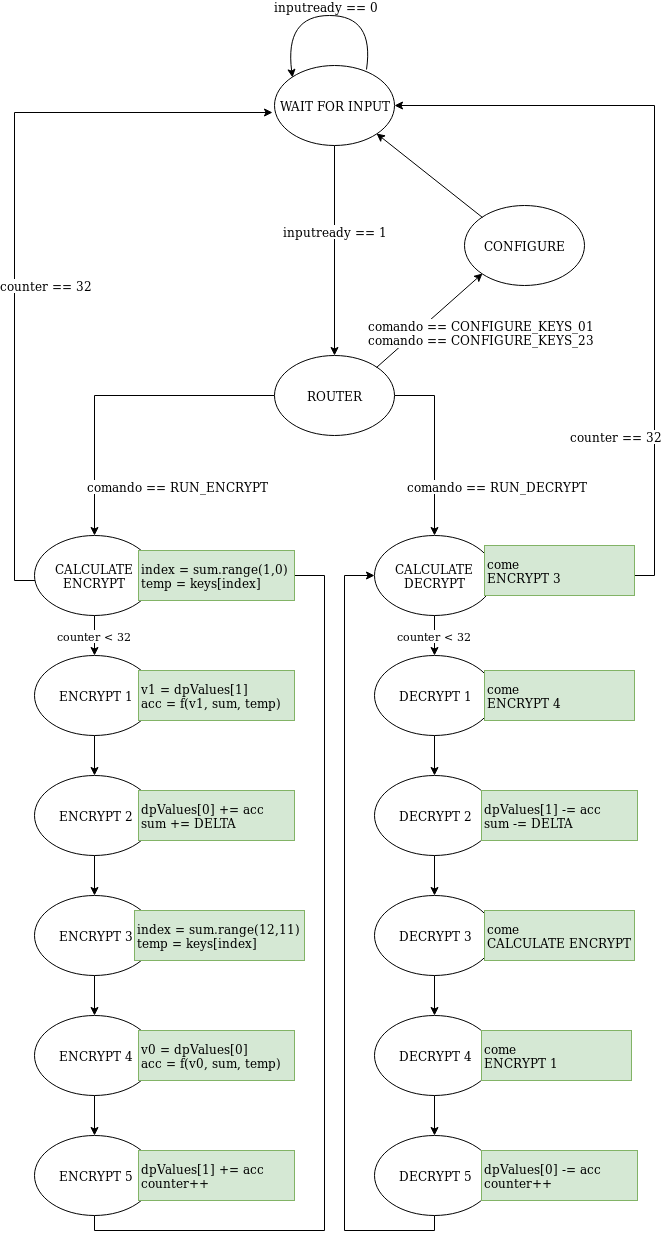
\includegraphics[width=0.48\textwidth]{vhdl_schemi/fsm.png}
    \caption{EFSM}
    \label{fig:efsm}
\end{figure}

\section{Simulazione con \textsf{Modelsim}}

\begin{figure*}[tb]
    \centering
    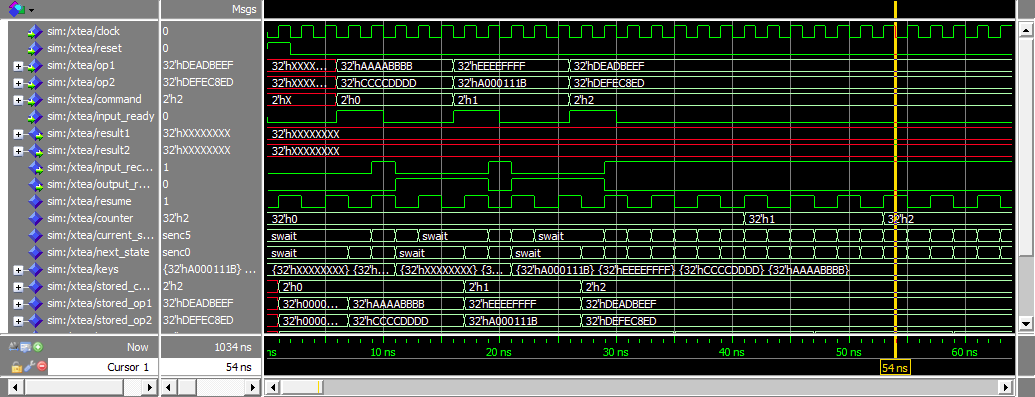
\includegraphics[width=\textwidth]{vhdl_schemi/modelsim.png}
    \caption{Porzione della simulazione. La fase di reset parte a 0ns. Le fasi di configurazione della prima e della seconda parte delle chiavi partono a 6ns e 16ns. La fase di criptazione del messaggio parte a 21ns.}
    \label{fig:modelsim}
\end{figure*}

Per poter simulare il progetto col software \textsf{Mentor Modelsim} creiamo un nuovo progetto all'interno del quale importiamo i file \code{xtea.vhd} e \code{xtea_helper.vhd}. Nella console digitiamo i comandi:
\begin{minted}[fontsize=\footnotesize]{tcl}
# Compilazione del file e visualizzazione report
vcom -reportprogress 300 -work work C:/percorso/xtea.vhd
# Apertura software di simulazione
vsim [-wlf output_waveform_file.wlf] work.xtea
do stimuli.do
# Chiusura simulazione
quit -sim
\end{minted}

Segue una parte del file \code{stimuli.do} che automatizza in parte il setup della simulazione. Il comando \code{force <porta> <valore> <tempo di assegnazione> ns} assegna al tempo voluto il valore alla porta. Così facendo possiamo comandare in modo molto immediato il nostro modulo. L'alternativa a questo sarebbe scrivere un file VHDL di testbench. 

Il metodo qui utilizzato ha una limitazione. Quando eseguiamo un'operazione, mettiamo \code{input_ready} alto, e poi lo abbassiamo quando viene segnalato \code{input_received}. Non avendo un'istruzione del tipo ``esegui fino a che \code{input_received = 1}" decidiamo di aspettare due cicli di clock, dopo i quali sappiamo dall'implementazione che tale segnale viene messo alto. Se però l'implementazione cambiasse allora questo sistema non funzionerebbe più.

Per questo nelle sezioni successive utilizziamo un modulo testbench, che permette una simulazione più ``robusta". 

\AtBeginEnvironment{minted}{%
  \renewcommand{\fcolorbox}[4][]{#4}}
\begin{minted}[fontsize=\footnotesize]{tcl}
# fai ripartire la simulazione (se non lo fai, 
# continua dal punto nel quale si era fermato)
restart -f 

# tolgo e ri-aggiungo i segnali del modulo alla schermata
delete wave *
add wave *

# RESET DEL MODULO
# il clock parte con 0, resta basso 1ns, viene alzato, 
# resta alto 1ns, e ripeto il processo ogni 2ns
force clock 0 0 ns, 1 1 ns -repeat 2
force reset 1 0 ns, 0 2 ns
force input_ready 0 0 ns
run 10ns

# CONFIGURAZIONE PRIMA PARTE DELLE CHIAVI
# i segnali che dico partire da 0ns non ripartono davvero
# dell'inizio ma dal punto in cui si era fermata la sim.
force op1 16#AAAABBBB 0 ns
force op2 16#CCCCDDDD 0 ns
force command 2#00    0 ns
force input_ready 1   0 ns
run 4 ns
force input_ready 0   
run 6 ns
\end{minted}

Il software permette di salvare le forme d'onda nel formato proprietario \code{wlf}. Una porzione di questa è visibile in Figura~\ref{fig:modelsim}. All'occorrenza, questo può essere convertito nel formato aperto \code{vcd} con il tool \code{wlf2vcd}. Il risultato può essere visto con il software \textsf{Gtkwave}. 

